\chapter{PHÂN TÍCH BÀI TOÁN VÀ YÊU CẦU}

\section{Bối cảnh và mục tiêu khảo sát}

Đề tài được đặt trong bối cảnh một nhóm marketing quản lý nhiều sản phẩm trên nhiều kênh truyền thông. Công việc không chỉ là tạo nội dung; nhóm còn phải lưu thông tin sản phẩm, lập kế hoạch, phân công, kiểm soát ngân sách, duyệt nội dung, lập lịch và theo dõi số liệu. Vì vậy, hệ thống cần giải quyết đồng thời các bài toán dữ liệu, quy trình và phân quyền.

Nếu chỉ trình bày sản phẩm hoặc một màn hình AI, người đọc chưa thấy được toàn bộ nghiệp vụ. Báo cáo này bắt đầu từ câu hỏi: \textbf{ai sử dụng hệ thống, họ cần làm những việc gì, dữ liệu nào đi qua từng bước và điều kiện nào để một bước được coi là hoàn thành}. Danh mục dưới đây dùng mã P01--P26 để truy vết yêu cầu; đây không phải danh sách bài tập hay 26 tính năng độc lập. Một yêu cầu lớn có thể bao gồm thao tác thêm, sửa, tìm kiếm và các quy tắc kiểm tra dữ liệu.

\section{Đối tượng sử dụng và trách nhiệm}

\begin{table}[h!]
\centering
\small
\caption{Đối tượng sử dụng và trách nhiệm trong hệ thống}
\begin{tabularx}{\textwidth}{|L{3.0cm}|Y|Y|}
\hline
\textbf{Đối tượng} & \textbf{Trách nhiệm chính} & \textbf{Quyền quyết định}\\\hline
Marketing Manager & Quản lý người dùng, nhóm sản phẩm, sản phẩm, kênh, chiến dịch, ngân sách; kiểm tra và duyệt nội dung. & Được duyệt hoặc từ chối nội dung; được điều chỉnh dữ liệu nền và quyền người dùng.\\\hline
Marketer & Xem chiến dịch được phân công, soạn nội dung, yêu cầu AI hỗ trợ, lập lịch theo quyền và nhập số liệu. & Được sửa bản nháp và gửi duyệt; không được duyệt nội dung của chính quy trình.\\\hline
Hệ thống Python & Kiểm tra đăng nhập, quyền, dữ liệu, khóa ngoại, trạng thái và điều phối giao dịch SQL. & Làm theo quy tắc đã lập trình; không tự quyết định thay Manager.\\\hline
AI service & Nhận context đã được chọn để gợi ý, tạo bản thảo hoặc tóm tắt số liệu. & Không phải actor nghiệp vụ; không được cấp quyền, đổi ngân sách, duyệt hoặc xuất bản.\\\hline
\end{tabularx}
\end{table}

\subsection*{Các quyết định nghiệp vụ dùng để giữ đúng phạm vi}

Trong bản thiết kế hiện tại, Manager xem được toàn bộ dữ liệu, tạo dữ liệu nền, đặt ngân sách, phân công và duyệt nội dung. Marketer chỉ xem chiến dịch được giao, tạo hoặc sửa bản nháp, gửi duyệt, đề xuất lịch cho nội dung đã được duyệt và nhập số liệu; Marketer không đổi ngân sách và không được duyệt nội dung. Hệ thống không tự xuất bản lên mạng xã hội.

Một chiến dịch hiện gắn với một sản phẩm và một người phụ trách để mô hình dễ kiểm tra; một chiến dịch có thể có nhiều nội dung nhưng mỗi nội dung gắn một kênh. Ngân sách dự kiến được lưu riêng với chi phí thực tế trong bảng chỉ số. Nếu nghiệp vụ cần nhiều sản phẩm hoặc nhiều người phụ trách, đó là phần mở rộng phải bổ sung bảng liên kết và ca kiểm thử, không tự đưa vào phạm vi hiện tại.

\section{Danh mục yêu cầu nghiệp vụ và quy tắc}

Danh mục này gom các yêu cầu nghiệp vụ chính và các quy tắc cần kiểm tra, gồm dữ liệu đầu vào, kết quả cần có và người chịu trách nhiệm. Mã \texttt{P01--P26} được dùng để đối chiếu với BFD, yêu cầu chức năng, bảng dữ liệu và ca kiểm thử. Các kiểm tra nhỏ như dữ liệu trùng, điều kiện xóa, lý do từ chối và xử lý lỗi được ghi như quy tắc của luồng liên quan, không tách thành một bài riêng.

\begingroup
\scriptsize
\setlength{\LTleft}{0pt}
\setlength{\LTright}{0pt}
\begin{longtable}{|C{0.8cm}|L{4.1cm}|C{1.8cm}|L{4.1cm}|L{3.7cm}|}
\caption{Danh mục yêu cầu nghiệp vụ và quy tắc cần giải quyết}\label{tab:problem-catalog}\\
\hline
\textbf{Mã} & \textbf{Yêu cầu nghiệp vụ / quy tắc} & \textbf{Chủ thể} & \textbf{Đầu vào / xử lý} & \textbf{Kết quả cần có}\\
\hline\endfirsthead
\multicolumn{5}{c}{\tablename\ \thetable{} -- tiếp theo}\\
\hline
\textbf{Mã} & \textbf{Yêu cầu nghiệp vụ / quy tắc} & \textbf{Chủ thể} & \textbf{Đầu vào / xử lý} & \textbf{Kết quả cần có}\\
\hline\endhead
\texttt{P01} & Tạo và quản lý tài khoản & Manager & Email, họ tên, vai trò; kiểm tra email duy nhất. & Tài khoản hoạt động hoặc lỗi trùng.\\\hline
\texttt{P02} & Đăng nhập hệ thống & Cả hai & Email và mật khẩu; kiểm tra giá trị băm. & Phiên đăng nhập hoặc lỗi 401.\\\hline
\texttt{P03} & Phân quyền theo vai trò & Hệ thống & Token và vai trò Manager/Marketer. & Cho phép hoặc từ chối endpoint.\\\hline
\texttt{P04} & Quản lý nhóm sản phẩm & Manager & Tên nhóm, mô tả; kiểm tra không trùng. & Bản ghi nhóm sản phẩm.\\\hline
\texttt{P05} & Quản lý sản phẩm & Manager & Tên, giá, USP, đối tượng, nhóm; kiểm tra FK và giá không âm. & Bản ghi sản phẩm thuộc đúng nhóm.\\\hline
\texttt{P06} & Quản lý kênh marketing & Manager & Tên kênh và quy tắc định dạng. & Kênh có cấu hình dùng cho nội dung.\\\hline
\texttt{P07} & Tạo chiến dịch & Manager & Tên, sản phẩm, mục tiêu, thời gian, ngân sách. & Chiến dịch ở trạng thái DRAFT.\\\hline
\texttt{P08} & Kiểm tra thời gian và ngân sách & Hệ thống & Ngày bắt đầu, ngày kết thúc, ngân sách. & Không nhận ngày ngược hoặc tiền âm.\\\hline
\texttt{P09} & Phân công người vận hành & Manager & Chiến dịch và người phụ trách. & Marketer nhìn thấy đúng chiến dịch.\\\hline
\texttt{P10} & Tạo bản nháp thủ công & Marketer & Chiến dịch, kênh, tiêu đề và nội dung. & Nội dung DRAFT.\\\hline
\texttt{P11} & Sửa và lưu bản nháp & Marketer & Nội dung đang soạn và người sửa. & Bản ghi được cập nhật, giữ trạng thái phù hợp.\\\hline
\texttt{P12} & Theo dõi nguồn bản nháp & Hệ thống & Người tạo, thời gian, provider và source\_ids. & Biết nội dung do người hay AI tạo.\\\hline
\texttt{P13} & Gửi nội dung để duyệt & Marketer & Bản DRAFT hoặc AI\_DRAFT đủ trường. & Chuyển sang PENDING.\\\hline
\texttt{P14} & Duyệt nội dung & Manager & Nội dung PENDING và quyết định duyệt. & APPROVED hoặc yêu cầu sửa.\\\hline
\texttt{P15} & Từ chối có lý do & Manager & Nội dung PENDING và lý do từ chối. & REJECTED kèm lý do.\\\hline
\texttt{P16} & Lập lịch nội dung & Người có quyền & Nội dung APPROVED, thời điểm, múi giờ. & Bản ghi lịch PLANNED.\\\hline
\texttt{P17} & Hủy hoặc ghi nhận lịch & Người có quyền & Lịch và trạng thái thực hiện. & CANCELLED hoặc EXECUTED.\\\hline
\texttt{P18} & Nhập số liệu theo ngày và kênh & Marketer & Views, Clicks, Conversions, Cost, Revenue. & Bản ghi chỉ số không âm.\\\hline
\texttt{P19} & Tính KPI & Hệ thống & Chỉ số đã lưu theo chiến dịch/kênh/ngày. & CTR, CPC, CPA, ROI; không chia cho 0.\\\hline
\texttt{P20} & Xem dashboard và báo cáo & Cả hai & Khoảng thời gian, chiến dịch, kênh. & Tổng hợp số liệu, bảng và biểu đồ.\\\hline
\texttt{P21} & Tìm kiếm dữ liệu & Cả hai & Từ khóa tên sản phẩm, chiến dịch, nội dung. & Danh sách phù hợp, có phân trang.\\\hline
\texttt{P22} & Lọc và sắp xếp & Cả hai & Trạng thái, ngày, kênh, chi phí. & Kết quả đúng điều kiện và thứ tự.\\\hline
\texttt{P23} & Kiểm tra dữ liệu trùng và xóa & Hệ thống & Khóa duy nhất, quan hệ FK, yêu cầu xóa. & Giữ dữ liệu hợp lệ, báo lỗi quan hệ.\\\hline
\texttt{P24} & Xử lý lỗi người dùng và lỗi hệ thống & Hệ thống & Dữ liệu sai, token hết hạn, thiếu bản ghi. & Mã lỗi rõ, không làm mất bản nháp.\\\hline
\texttt{P25} & Gợi ý và tạo nội dung bằng AI & Marketer/Manager & Context từ SQL, mục tiêu và quy tắc kênh. & Kết quả AI\_DRAFT có schema và nguồn.\\\hline
\texttt{P26} & Tóm tắt số liệu và xử lý AI lỗi & AI service & Số liệu đã lọc; timeout, 429, JSON sai hoặc offline. & Tóm tắt có nguồn hoặc lỗi có thể thử lại; không tự xuất bản.\\\hline
\end{longtable}
\endgroup

\section{Quy trình nghiệp vụ từ đầu đến cuối}

\begin{enumerate}
  \item \textbf{Chuẩn bị dữ liệu}: Manager tạo tài khoản, nhóm sản phẩm, sản phẩm và kênh. Sản phẩm phải có giá, USP, đối tượng và nhóm tham chiếu.
  \item \textbf{Lập chiến dịch}: Manager chọn sản phẩm, nhập mục tiêu, thời gian, ngân sách và người phụ trách. Hệ thống kiểm tra ngày, tiền và khóa ngoại.
  \item \textbf{Tạo nội dung}: Marketer tạo bản nháp thủ công hoặc gọi AI. Nội dung ghi rõ chiến dịch, kênh, người tạo và nguồn context.
  \item \textbf{Kiểm duyệt}: Marketer kiểm tra và gửi PENDING. Manager xem nội dung, dữ liệu nguồn và chuyển APPROVED hoặc REJECTED kèm lý do.
  \item \textbf{Lập lịch}: Chỉ nội dung APPROVED mới được tạo lịch. Hệ thống lưu thời điểm dự kiến và trạng thái.
  \item \textbf{Đo lường}: Marketer nhập Views, Clicks, Conversions, Cost và Revenue theo ngày/kênh.
  \item \textbf{Báo cáo}: Hệ thống tính KPI, lọc và tổng hợp dashboard. AI có thể tóm tắt kết quả nhưng không thay công thức SQL/Python.
\end{enumerate}

\section{Yêu cầu chức năng}

\begin{table}[h!]
\centering
\scriptsize
\caption{Đặc tả yêu cầu chức năng theo đầu vào, xử lý và đầu ra}
\begin{tabularx}{\textwidth}{|C{0.8cm}|L{2.7cm}|L{3.0cm}|L{3.7cm}|Y|}
\hline
\textbf{Mã} & \textbf{Chức năng} & \textbf{Đầu vào} & \textbf{Xử lý chính} & \textbf{Đầu ra}\\\hline
FR01 & Đăng nhập, phân quyền & Email, mật khẩu, token & Xác thực, tạo JWT, kiểm tra vai trò & Phiên hoặc lỗi 401/403\\\hline
FR02 & Nhóm sản phẩm & Tên, mô tả & Kiểm tra duy nhất và CRUD & Danh sách nhóm\\\hline
FR03 & Sản phẩm & Nhóm, tên, giá, USP, đối tượng & Kiểm tra FK, giá không âm & Bản ghi sản phẩm\\\hline
FR04 & Kênh marketing & Tên, quy tắc định dạng & Kiểm tra tên duy nhất & Danh sách kênh\\\hline
FR05 & Chiến dịch & Sản phẩm, mục tiêu, ngày, ngân sách, người phụ trách & Kiểm tra ngày, tiền, FK và trạng thái & Chiến dịch DRAFT/ACTIVE\\\hline
FR06 & Nội dung & Chiến dịch, kênh, tiêu đề, body, CTA & Lưu bản nháp, nguồn và trạng thái & Nội dung DRAFT/AI\_DRAFT\\\hline
FR07 & Kiểm duyệt & Nội dung, quyết định, lý do & Manager kiểm tra PENDING & APPROVED/REJECTED\\\hline
FR08 & Lịch đăng & Nội dung APPROVED, thời gian & Kiểm tra trạng thái và trùng lịch & Lịch PLANNED\\\hline
FR09 & Chỉ số và KPI & Views, Clicks, Conversions, Cost, Revenue & Lưu theo ngày/kênh và tính công thức & KPI, bảng và biểu đồ\\\hline
FR10 & Tìm kiếm, lọc, báo cáo & Từ khóa, trạng thái, thời gian & Truy vấn có tham số, phân trang, tổng hợp & Danh sách và dashboard\\\hline
FR11 & AI hỗ trợ marketing & Context đã chọn, yêu cầu người dùng & Gọi service, kiểm tra schema, lưu log & Ý tưởng, bản nháp hoặc tóm tắt\\\hline
\end{tabularx}
\end{table}

\section{Yêu cầu phi chức năng}

\begin{table}[h!]
\centering
\small
\caption{Đặc tả yêu cầu phi chức năng}
\begin{tabularx}{\textwidth}{|C{1.0cm}|L{3.1cm}|Y|L{3.1cm}|}
\hline
\textbf{Mã} & \textbf{Nhóm} & \textbf{Yêu cầu} & \textbf{Cách kiểm tra}\\\hline
NFR01 & Bảo mật & Mật khẩu lưu dạng băm; JWT secret và API key lấy từ môi trường; endpoint duyệt yêu cầu Manager. & Thử sai mật khẩu, sai vai trò và rà soát cấu hình.\\\hline
NFR02 & Toàn vẹn dữ liệu & PK, FK, UNIQUE, CHECK không âm và điều kiện ngày phải được khai báo trong SQL. & Chạy dữ liệu sai và kiểm tra lỗi.\\\hline
NFR03 & Hiệu năng & Truy vấn danh sách có phân trang; mục tiêu CRUD dưới 150 ms trong dữ liệu mẫu. & Đo bằng log trong cùng môi trường.\\\hline
NFR04 & Dễ sử dụng & Người dùng nhìn thấy trạng thái, lỗi, nguồn bản nháp và thao tác tiếp theo. & Kiểm tra luồng đăng nhập, CRUD, duyệt và báo cáo.\\\hline
NFR05 & Chịu lỗi & API có timeout, xử lý 429, JSON sai, provider offline và giữ bản nháp cũ. & Mock từng lỗi và đối chiếu log.\\\hline
NFR06 & Bảo trì & Tách module Python, dùng SQL rõ ràng, cấu hình ngoài mã nguồn và có README. & Rà soát cây thư mục và hướng dẫn chạy.\\\hline
NFR07 & Sao lưu và khôi phục & DDL, seed và dữ liệu mẫu có thể tạo lại; hướng dẫn sao lưu CSDL và kiểm tra phục hồi. & Chạy quy trình backup/restore trên môi trường demo.\\\hline
\end{tabularx}
\end{table}

\section{Actor, Use Case và ma trận quyền}

\subsection{Ma trận quyền}

\begin{table}[h!]
\centering
\small
\caption{Ma trận quyền giữa Marketing Manager và Marketer}
\begin{tabularx}{\textwidth}{|L{3.0cm}|Y|C{1.8cm}|C{1.8cm}|}
\hline
\textbf{Phân hệ} & \textbf{Hành động} & \textbf{Manager} & \textbf{Marketer}\\\hline
Tài khoản & Đăng nhập và xem phiên & Có & Có\\\hline
Tài khoản & Tạo tài khoản và đổi vai trò & Có & Không\\\hline
Nhóm/sản phẩm & Thêm, sửa, xóa & Có & Xem\\\hline
Kênh & Thêm, sửa và cấu hình quy tắc & Có & Xem\\\hline
Chiến dịch & Tạo, sửa, ngân sách và phân công & Có & Xem chiến dịch được giao\\\hline
Nội dung & Tạo, sửa và gửi duyệt & Có & Có\\\hline
Nội dung & Duyệt hoặc từ chối có lý do & Có & Không\\\hline
Lịch & Tạo, hủy và ghi nhận lịch & Có & Có theo quyền\\\hline
Chỉ số & Nhập số liệu và xem dashboard & Có & Có\\\hline
AI & Yêu cầu gợi ý, bản thảo, tóm tắt & Có & Có\\\hline
\end{tabularx}
\end{table}

\subsection{Sơ đồ Use Case}

\begin{figure}[h!]
\centering
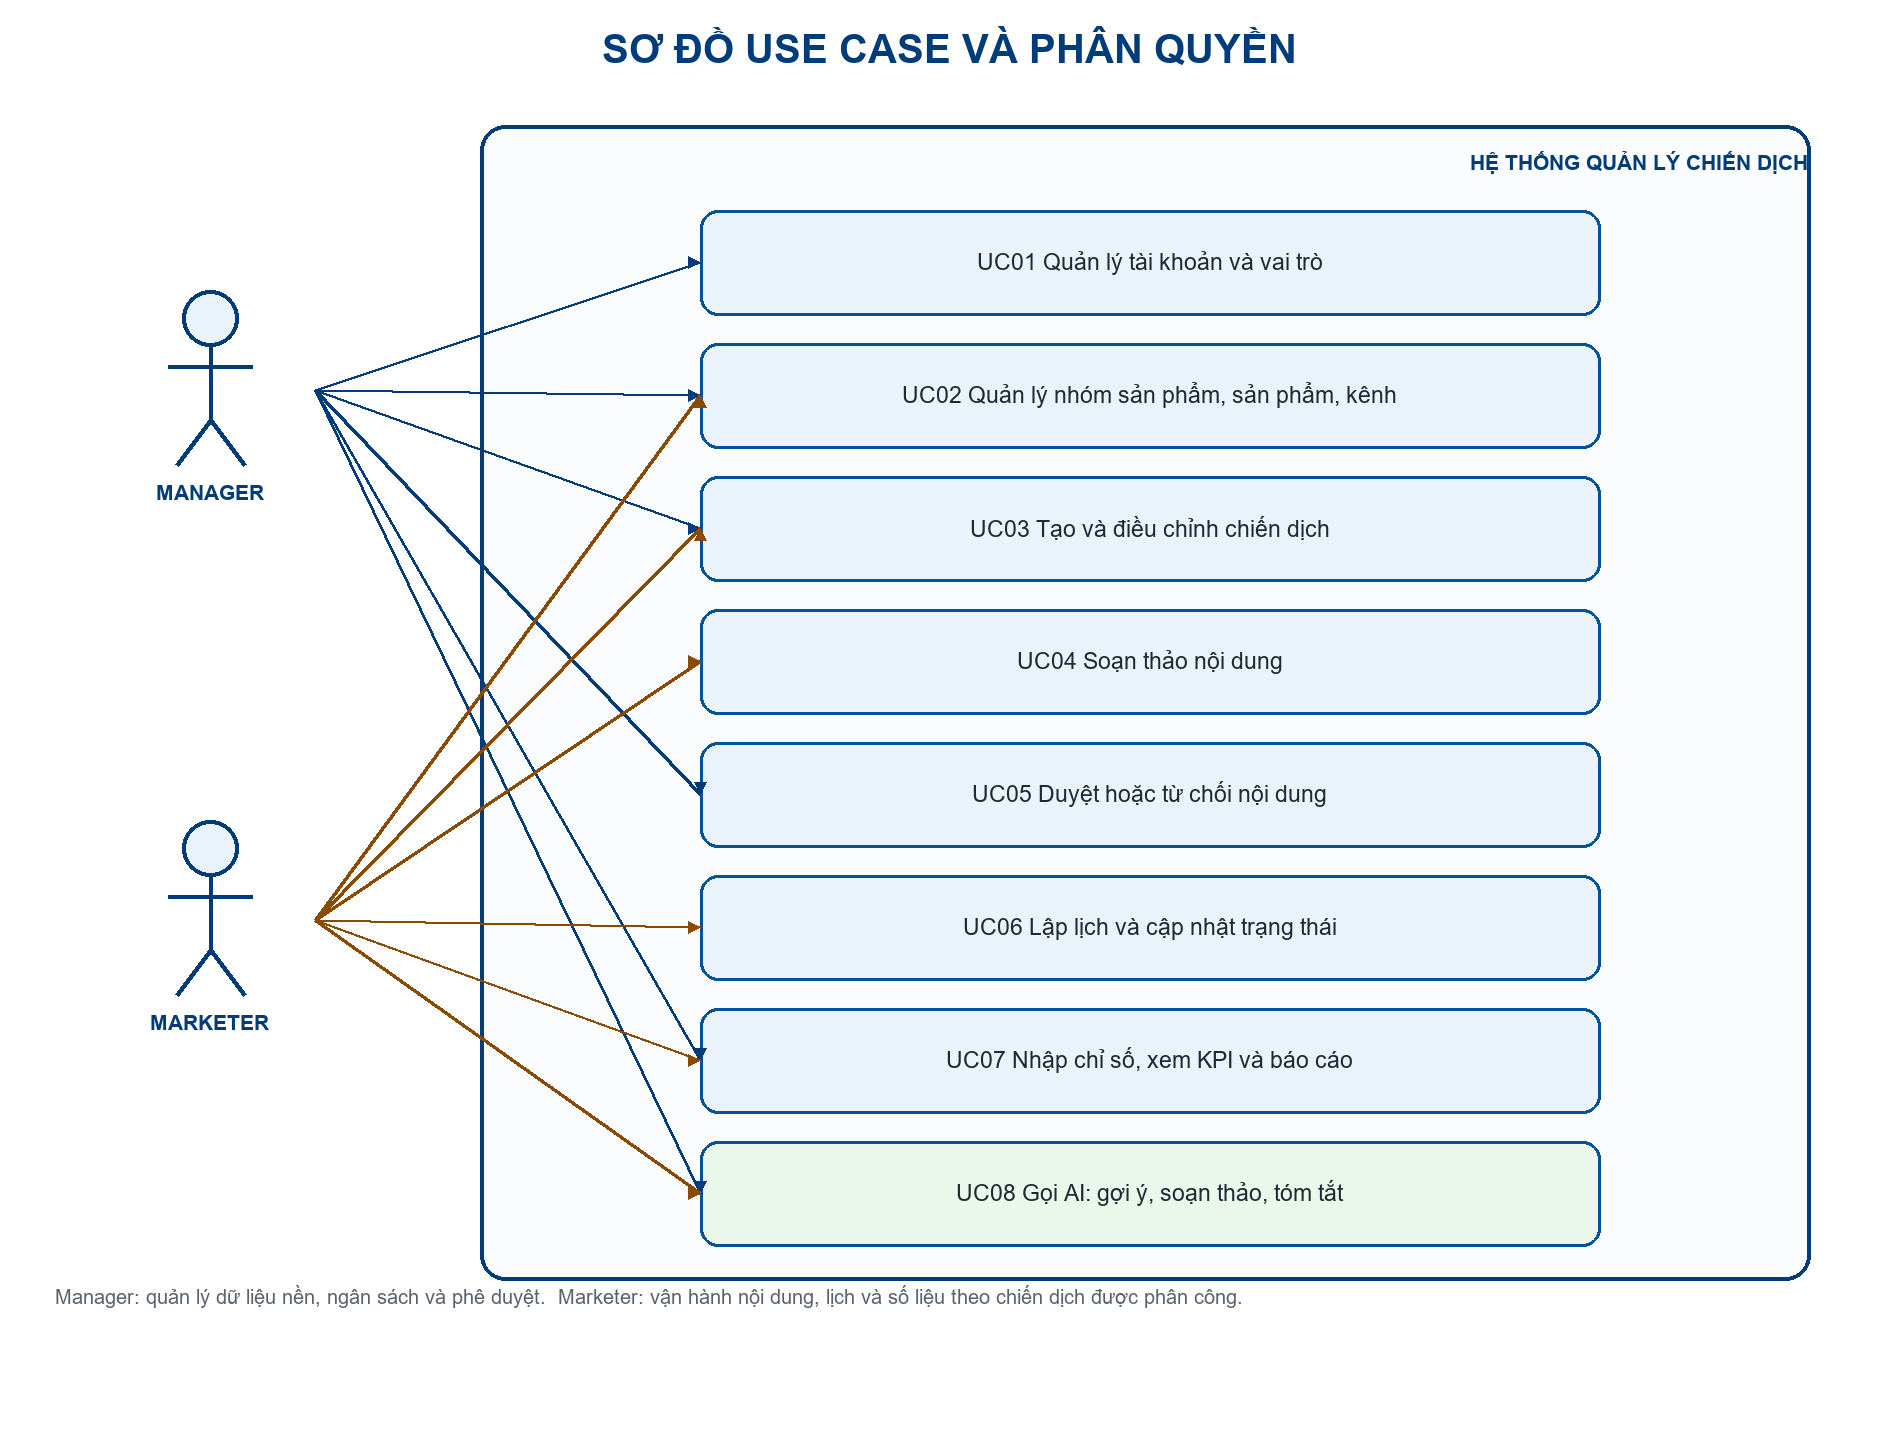
\includegraphics[width=0.96\textwidth]{images/usecase.png}
\caption{Sơ đồ Use Case và ranh giới trách nhiệm của hai actor}
\end{figure}

Sơ đồ trên phân biệt rõ hai người dùng. Manager chịu trách nhiệm dữ liệu nền, ngân sách và duyệt; Marketer vận hành nội dung, lịch và số liệu. AI chỉ xuất hiện như một chức năng được gọi trong luồng, không phải người dùng có quyền riêng.

\section{Đầu vào, đầu ra và điều kiện hoàn thành}

\begin{table}[h!]
\centering
\small
\caption{Đầu vào và đầu ra của các nhóm nghiệp vụ}
\begin{tabularx}{\textwidth}{|L{3.0cm}|Y|Y|Y|}
\hline
\textbf{Nhóm} & \textbf{Đầu vào} & \textbf{Xử lý} & \textbf{Đầu ra/điều kiện hoàn thành}\\\hline
Dữ liệu nền & Tài khoản, nhóm, sản phẩm, kênh & Kiểm tra bắt buộc, duy nhất và FK & Dữ liệu có thể dùng để lập chiến dịch.\\\hline
Chiến dịch & Sản phẩm, mục tiêu, ngày, ngân sách, người phụ trách & Kiểm tra quy tắc và lưu trạng thái & Chiến dịch được phân công.\\\hline
Nội dung & Kênh, bản nháp, quyết định duyệt & Lưu phiên bản, chuyển trạng thái & APPROVED trước khi lập lịch.\\\hline
Đo lường & Chỉ số theo ngày/kênh & Kiểm tra không âm và tính KPI & Dashboard có số liệu truy vết được.\\\hline
AI & Context từ bảng SQL, yêu cầu cụ thể & Gọi AI, kiểm tra JSON, người duyệt & Bản nháp/tóm tắt có nguồn; không tự xuất bản.\\\hline
\end{tabularx}
\end{table}

\enlargethispage{4\baselineskip}
\section{Kết luận chương}

Chương này hoàn thành việc xác định phạm vi, hai actor, 26 mã yêu cầu nghiệp vụ và quy tắc, yêu cầu chức năng và phi chức năng, quy trình đầu-cuối, đầu vào/đầu ra và điều kiện hoàn thành. Danh mục \texttt{P01--P26} được dùng xuyên suốt các chương tiếp theo để phân rã chức năng, tạo bảng SQL, dựng ERD và kiểm thử; cơ sở dữ liệu không được thiết kế tách rời khỏi yêu cầu đã khảo sát.
